\documentclass[../main.tex]{subfiles}
\graphicspath{{figures/}{../figures/}}

\begin{document}
% \todo[color=green!40]{完成问题四模型的求解(sections/q4\_solution)}

\noindent \textbf{步骤 1:初始化系统参数与几何约束}

设定导弹、无人机、防御目标及烟幕云团的物理参数,构建三维空间中的动态运动模型与几何关系,并通过经验与物理限制为优化变量设定合理边界。

\noindent \textbf{步骤 2:构建多无人机协同遮蔽动态仿真模型} 

建立三维空间中导弹与目标之间的视线向量模型,结合无人机投放烟幕的空间分布,采用时间离散化对整个过程进行精细化推进,每一时刻判断视线段是否与至少一个有效烟幕区域发生空间重叠。根据当前优化参数,在仿真时序中同步更新三架无人机的烟幕释放状态及其空间覆盖范围。逐时刻调用几何遮挡判定函数,判断是否实现对导弹视线的完全遮蔽。

\noindent \textbf{步骤 3:构建优化目标函数并调用差分进化算法} 

利用差分进化算法自动完成初始化种群、变异、交叉、选择、迭代进化等步骤,利用差分进化算法全局搜索最优参数组合。


\noindent \textbf{步骤 4:输出最优遮蔽方案与部署参数} 

解析优化结果,输出可执行的无人机投放策略和预期效果。

\begin{figure}[H]
\centering
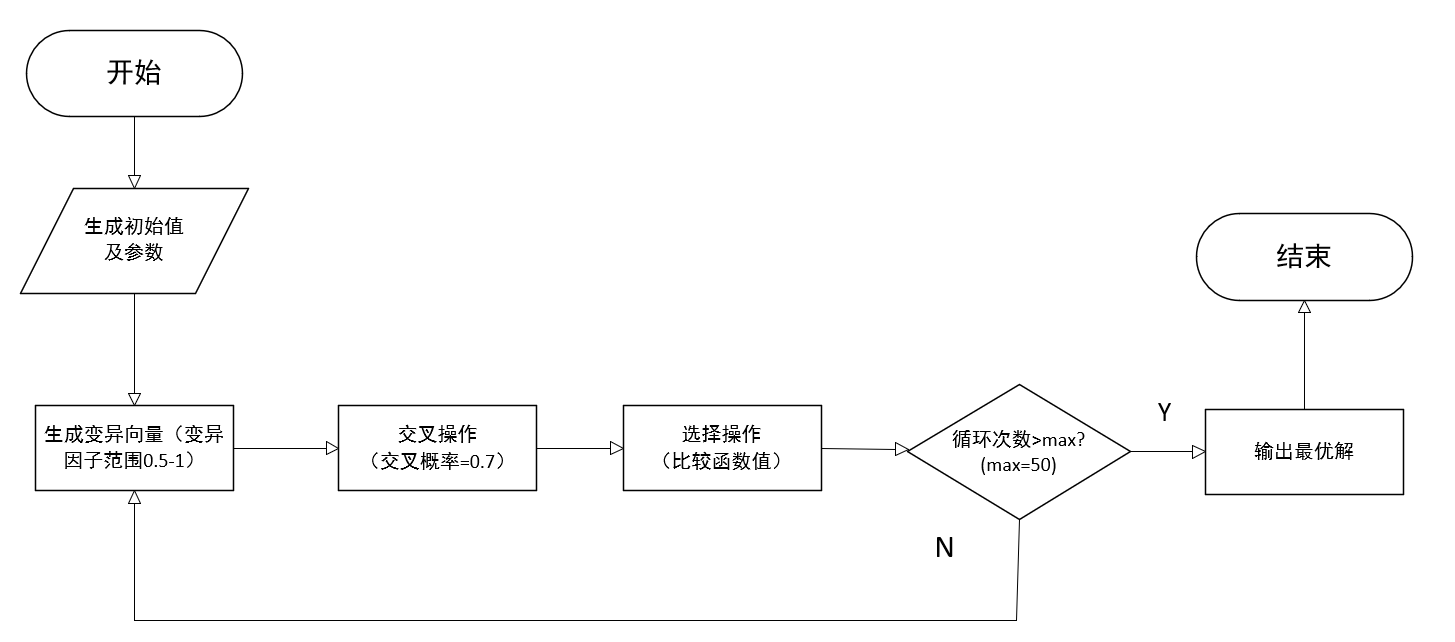
\includegraphics[scale=0.35]{问题4流程图.png}
\caption{问题四模型求解流程图}
\label{图...---2}
\end{figure}

按照上述算法思路,利用Pytho求解得到\textbf{最大有效时间为11.50s},具体参数见表\ref{tab:--001}和表\ref{tab:---031} .

\begin{table}[H]
\caption{问题4投放策略-1}
\label{tab:--001} 
\centering
\begin{small}
\begin{tabular}{ccccc}
\toprule[1.5pt]
无人机编号 &无人机运动方向 & 无人机运动速度  & 烟幕干扰弹投放点的x坐标& 烟幕干扰弹投放点的y坐标 \\
\midrule[1pt]
FY1 & 4.86             &  96.37                    & 17855.44                    & 4.72     \\            
FY2 & 246.86           &  87.25                    & 11643.20                    & 565.03      \\           
FY3 & 100.85           &  93.93                    & 5505.75                    & -420.55      \\           
\bottomrule[1.5pt]
\end{tabular}
\end{small}
\end{table}

\begin{table}[H]
\caption{问题4投放策略-2}
\label{tab:---031} 
\centering
\begin{small}
\begin{tabular}{ccccc}
\toprule[1.5pt]
    干扰弹投放点的z坐标 &干扰弹起爆点的x坐标&干扰弹起爆点的y坐标&干扰弹起爆点的z坐标&有效干扰时长\\
\midrule[1pt]
1800.00             & 17905.80                 & 9.00     & 1798.65                    & 4.60  \\               
1400.00             & 11405.11                 & 7.84     & 1163.68                    & 2.95  \\               
700.00              & 5411.79                  & 69.82    & 561.54                    & 3.10  \\                
\bottomrule[1.5pt]
\end{tabular}
\end{small}
\end{table}
在表\ref{tab:--001}和表\ref{tab:---031}条件下,某一有效时刻导弹和烟幕云团的遮挡示意图,如图\ref{图----3}所示.

\begin{figure}[H]
\centering
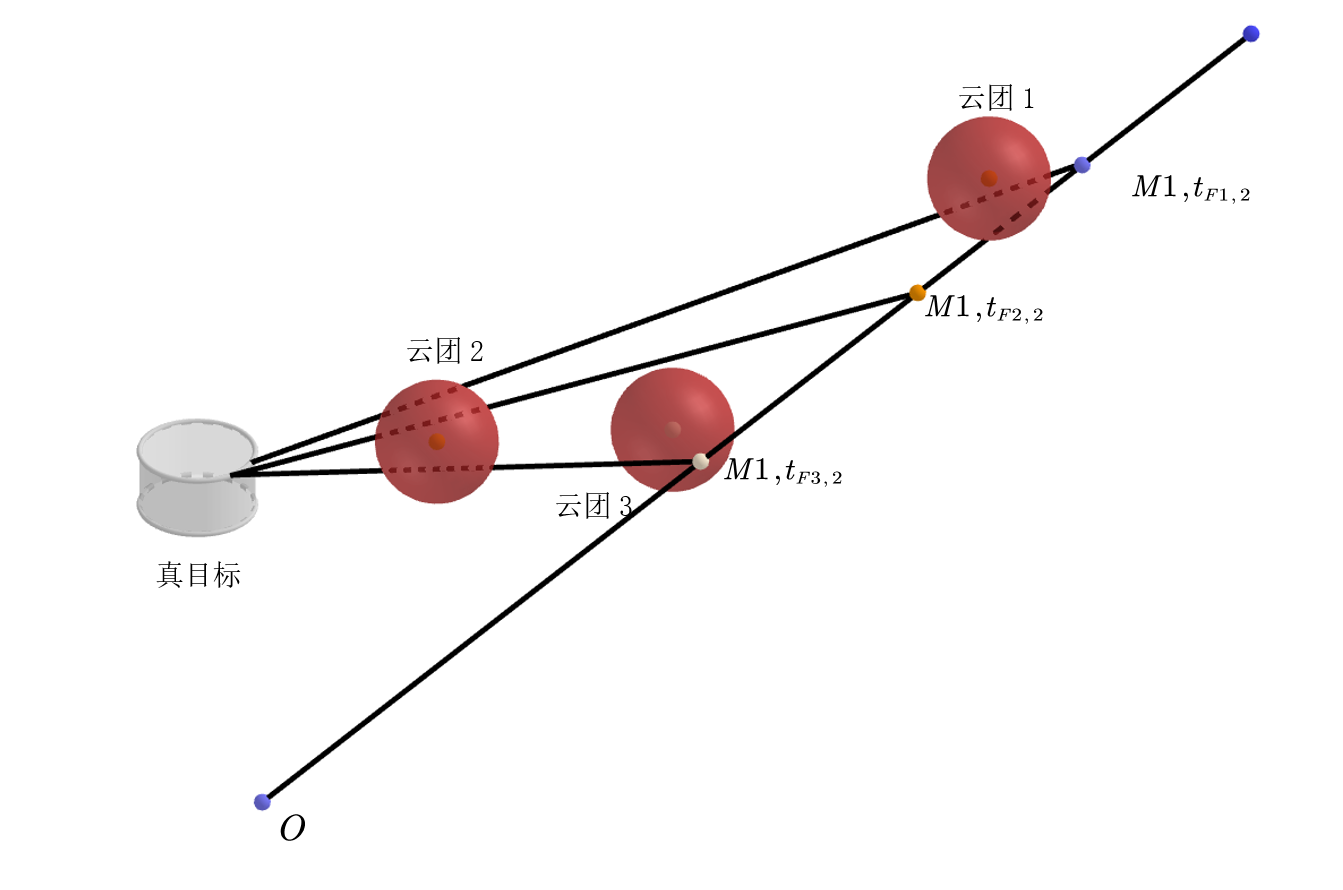
\includegraphics[scale=0.5]{图三.png}
\caption{}
\label{图----3}
\end{figure}




















\end{document}